% MIT License

% Copyright (c) 2022 Chiyuru

% Permission is hereby granted, free of charge, to any person obtaining a copy of this software and associated documentation files (the "Software"), 
% to deal in the Software without restriction, including without limitation the rights
% to use, copy, modify, merge, publish, distribute, sublicense, and/or sell
% copies of the Software, and to permit persons to whom the Software is
% furnished to do so, subject to the following conditions:

% The above copyright notice and this permission notice shall be included in all copies or substantial portions of the Software.

% THE SOFTWARE IS PROVIDED "AS IS", WITHOUT WARRANTY OF ANY KIND, EXPRESS OR IMPLIED, INCLUDING BUT NOT LIMITED TO THE WARRANTIES OF MERCHANTABILITY,
% FITNESS FOR A PARTICULAR PURPOSE AND NONINFRINGEMENT. IN NO EVENT SHALL THE AUTHORS OR COPYRIGHT HOLDERS BE LIABLE FOR ANY CLAIM, DAMAGES OR OTHER
% LIABILITY, WHETHER IN AN ACTION OF CONTRACT, TORT OR OTHERWISE, ARISING FROM,
% OUT OF OR IN CONNECTION WITH THE SOFTWARE OR THE USE OR OTHER DEALINGS IN THE SOFTWARE.

\documentclass[UTF8]{ctexart}

\usepackage{amssymb}
\usepackage{amsmath}
\usepackage{cases}
\usepackage{cite}
\usepackage{graphicx}
\usepackage[margin=1in]{geometry}
\geometry{a4paper}
\usepackage{fancyhdr}
\pagestyle{fancy}
\fancyhf{}


\title{学习算法报告}
\author{
    刘锦坤
    \\2022013352}
\date{\today}
\pagenumbering{arabic}

\begin{document}

\fancyhead[C]{学习算法报告}
\fancyfoot[C]{\thepage}

\maketitle
\tableofcontents

\section{问题1}

\begin{figure}[h]
    \centering
    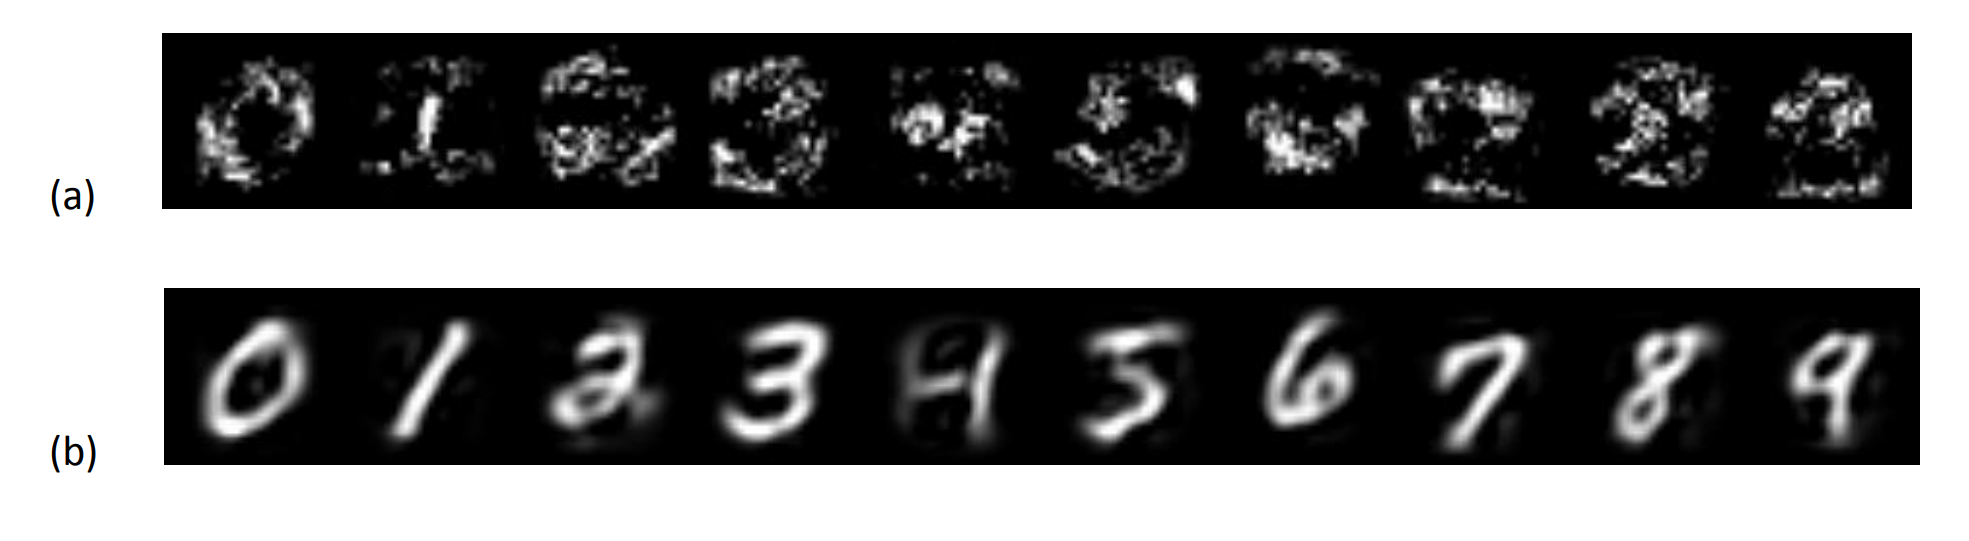
\includegraphics[width=0.8\textwidth]{./image/ab.png}
    \caption{Question1}
    \label{fig:Question1}
\end{figure}

\begin{figure}[h]
    \centering
    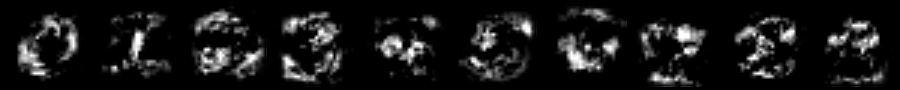
\includegraphics[width=0.8\textwidth]{./image/weights.png}
    \caption{weights.png}
    \label{fig:weights}
\end{figure}

\indent 根据生成的weights.png(如图\ref{fig:weights})可知,Question1中,图片(a)更能够代表感知机所学习到的权重矩阵。

\indent 可以看到,各个数字分类的权重向量在可视化后都呈现出对应的数字的轮廓的形状。这是因为对于每个输入数字,要能够将其通过Softmax Regression的方法将其正确分类,就需要其在输出层对应数字位置的值最大。在训练过程中,感知机根据输入的数字的特征,调整权重矩阵,使得输入数字的特征与其对应的权重矩阵的乘积最大,从而使得输出层对应数字位置的值最大。在这个问题中,每个输入的特征就是其各个像素点的值,因此在对应数字越可能出现的位置,权重中对应的值就越大,从而呈现出对应数字的轮廓的形状。

\indent 但是因为即使是对应同一个数字的各个输入中,手写的数字的形状也是有所不同的,因此权重矩阵在可视化后不会表现成一个完全锐利的数字轮廓,而是一个较为模糊的数字轮廓,其反映的事实上是对应数字的各个输入的特征的平均值,也即特定数字在训练的输入中最概然出现的那些位置,这也就导致对于某些输入,感知机可能会产生错误的分类判断。
\end{document}